\documentclass[../main.tex]{subfiles}

\begin{document}
	\section{Dynamics}
		\begin{preamb}
			In physics, forces change the state of motion of an object. Studying forces allow us to talk about the effects on the object and predict the motions of the object. In this chapter, we will look at two-dimensional dynamics.                         
		\end{preamb}
	
		\subsection{Forces}
		\pdef{Force}{A force is a push or pull on a body. The SI unit of force is the newton [\si{\newton}].}
		
		\subsection{Newton's Laws of Motion}
		The three laws of motion are:
		\pdef{First Law}{An object does not change its state of motion until being acted upon by a force. This is also known as the law of inertia.}
		\pdef{Second Law}{The net force \(F_\mathrm{net}\) acting on a body is given by as \[F = ma_\mathrm{net}\] where \(m\) is the mass of the body and \(a_\mathrm{net}\) is the net acceleration of the body.}
		\pdef{Third Law}{When two bodies interact, the forces on the bodies from each other are always equal in magnitude and opposite in direction.}
		
		\subsection{Effects of Forces}
		From the first law, we know that a force can accelerate a body (\textit{i.e.} change velocity). This can be done by either changing the magnitude or direction of the velocity vector of the body.
			
			\subsubsection{Static System}
			A body is said to be in translational equilibrium if the net force on the body is zero. This is sometimes called a static system, where no net acceleration takes place.
			
			When resolving statics problems, it is important to ensure all force vectors add up to zero. Graphically, all these vectors when placed tip to tail should end where they started.
			
			\subsubsection{Unbalanced System}
			If the net force on a body is not zero, the object is not in translational equilibrium, and that means its velocity is changing.
			
		
		\subsection{Types of Forces}
		It is not sufficient to just describe forces as ``push'' and ``pull'' forces. Different names for forces are designated for different contexts. In this syllabus, only friction is required, but I will add common forces as well. Refer to chapter 4 for weight.
		
			\subsubsection{Normal Force}
			\pdef{Normal Force}{The normal force is the force perpendicular to a surface that the surface applies to a body due to its compression.}
			\begin{center}
				\begin{tikzpicture}
					\draw (2,0) -- (2,1) -- (3,1) -- (3,0);
					\draw [line width=0.5mm, ->] (2.5,0.5) -- (2.5,-1.5) node[anchor=north] {\(mg\)};
					\draw [line width=0.5mm, ->] (2.6,0) -- (2.6,2) node[anchor=south] {\(N\)};
					\draw (0,0) -- (5,0) node[pos=1.0, anchor=north east] {surface};
				\end{tikzpicture}
			\end{center}
		
			\subsubsection{Tension}
			\pdef{Tension}{Tension is the force exerted in a body when it is pulled on.}
			On a massless string, the tension on the two ends are equal.
			\begin{center}
				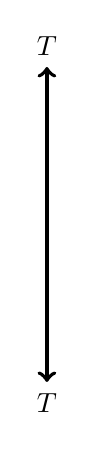
\begin{tikzpicture}
					\draw [line width=0.5mm, <-] (0,2) node[anchor=south] {\(T\)} -- (0,0) ;
					\draw [line width=0.5mm, ->] (0,0) -- (0,-2) node[anchor=north] {\(T\)};
				\end{tikzpicture}
			\end{center}
		
			\subsubsection{Friction}
			\pdef{Friction}{Friction is the force parallel to a surface that a surface applies to an body due to its roughness.}
			Friction is a resistive force, that works against a force applied. There are two types of friction: kinetic and static friction. Kinetic friction deals with two objects moving on each other, and exists when an object is moving, while static friction deals with two objects that are stationary. The maximum static friction is the minimum force to be applied to allow an object to start moving on a surface.
			\begin{center}
				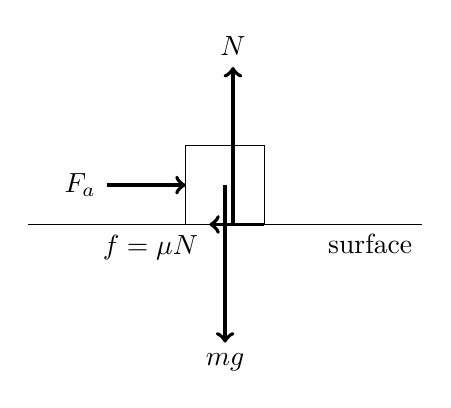
\begin{tikzpicture}
				\draw (2,0) -- (2,1) -- (3,1) -- (3,0);
				\draw [line width=0.5mm, ->] (2.5,0.5) -- (2.5,-1.5) node[anchor=north] {\(mg\)};
				\draw [line width=0.5mm, ->] (2.6,0) -- (2.6,2) node[anchor=south] {\(N\)};
				\draw [line width=0.5mm, ->] (1,0.5) node[anchor=east] {\(F_a\)} -- (2,0.5);
				\draw [line width=0.5mm, ->] (3,0) -- (2.3,0) node[anchor=north east] {\(f = \mu N\)}; 
				\draw (0,0) -- (5,0) node[pos=1.0, anchor=north east] {surface};
				\end{tikzpicture}
			\end{center}
			
\end{document}